\documentclass[a4paper,10pt]{article}
\usepackage{amsmath}
\usepackage{amsthm}
\newtheorem{mydef}{Definition}
\usepackage{url, hyperref}
\usepackage{amsthm}
\usepackage{amsfonts}
\usepackage{amssymb}
\newtheorem{theorem}{Theorem}
\newtheorem{lemma}{Lemma}
%\usepackage{fullpage}
\usepackage{tikz}
\usepackage{float}
\usepackage{listings}
\usepackage{color}
\usepackage{mathtools}
\usepackage[T1]{fontenc}
\usepackage{subfigure}
\usepackage{algorithm}
\usepackage{algpseudocode}
\bibliographystyle{plain}

\newenvironment{changemargin}[2]{%
\begin{list}{}{%
\setlength{\topsep}{0pt}%
\setlength{\leftmargin}{#1}%
\setlength{\rightmargin}{#2}%
\setlength{\listparindent}{\parindent}%
\setlength{\itemindent}{\parindent}%
\setlength{\parsep}{\parskip}%
}%
\item[]}{\end{list}}

\usepackage[linecolor=green!70!white,
backgroundcolor=blue!20!white,bordercolor=red]{todonotes}
\newcommand{\note}{\todo}

\begin{document}
\begin{titlepage}

\begin{changemargin}{-1cm}{-1cm}
\begin{center}

\begin{minipage}{1.2\textwidth}
\begin{center}
\vspace{2cm}
    {\Huge \bf Efficient segmentation algorithms for shark fin
identification }
\end{center}
\end{minipage}

\vspace{1.3cm}

\begin{minipage}{0.49\textwidth}
\begin{center} \LARGE
\emph{Author:}\\
L. Cilli\'{e}, 16010450
\end{center}
\end{minipage}
\begin{minipage}{0.49\textwidth}
\begin{center} \LARGE
\emph{Project Advisors:} \\
Prof. B.M. Herbst\\Dr. S.J Van der Walt

\end{center}
\end{minipage}

\vspace{1.3cm}
{\LARGE October 2013}

\end{center}

\vfill

\vspace{20mm}
\hfill{\LARGE Honours Project, Applied Mathematics}\hfill\,

\,\hfill{\LARGE Stellenbosch University}\hfill\,

\end{changemargin}

\end{titlepage}

\begin{abstract}
This project investigates the use of various segmentation algorithms as
  part of a larger pipeline for the identification of Great White sharks.
For this purpose, the Growcut algorithm is studied in detail.
A pipeline is developed containing various algorithms in aid of the
identification process.  The pipeline can be used to compare new shark fin
images with existing images in a database, establishing whether the shark is
already on the database or not.  This information can be used to determine a more accurate population estimate in a specific region,
thereby assisting in the conservation of the Great White shark.
\end{abstract}

\newpage
\tableofcontents

\newpage
\section{Problem statement and motivation}
\subsection{}
Just as humans are identified by their fingerprints, sharks have a unique
dorsal fin structure.  Identifying shark sightings is very
valuable for biological and ecological research.  Such information can be used to predict migration patterns, possible habitats and also in warning people about sharks in a certain area.  In order to identify the sharks and to compare various shark sightings,
images of
shark fins are analysed by a computer. 
This analysis consists of identifying the edges in the image and segmenting the
foreground, the shark, from the background, the sea. 
Although the images provided are of a good quality and have been cropped
to only include the fin, the
foreground and background properties can still vary significantly, making this a
non-trivial problem.  The approach consists of
evaluating (by means of a computer) different methods for classifying foreground
and background, as well as segmenting the foreground successfully.  \\

The project was conceived by a PhD
student in Marine Biology, Ms. S. Andreotti, who approached Dr. S.J. van der Walt for
help regarding a problem she encountered in her research, namely
how images of shark fins  can be used in identifying sharks, so that their
ecological and behavioural patterns can be studied more easily.
For this purpose, a database of shark fin images has been compiled.
To
draw reliable conclusions, images in the database must be in a form such that it can be compared to the new images.
The goal is to group images of a certain individual together.  We
already know that it is possible to categorize each image, because a
  human is able to group images based on the unique shape of the
dorsal fin.  To do so, one would have to find a way to match new
input data with existing images in the database.  To perform such a
  process manually is laborious. 
Since the student's 
focus is on the distribution and movements of sharks and not on developing new
software, an algorith that automates the task is a significant contribution. \\

Using such technology, the Great White shark population and migration
patterns can be studied in a way that is not harmful to
the sharks, since the sharks need not to be tagged manually. Thereby
contributing in their conservation of sharks and the environment.  

\newpage
Below are a few examples of the data used in this research project.  
The database consists of various shark fin images, taken on different dates and
at different locations.
Also note that some sharks are
  represented more than once, i.e. the database
might contain two or more images of the same shark.

\note{Kan jy eerder 'n subfigure gebruik hier?  Dan hoef jy ook nie bo 'n
  manual newpage in te sit nie.  Ek gebruik dan subfigures???}
\begin{figure}[H]
\centering
\mbox{\subfigure[]{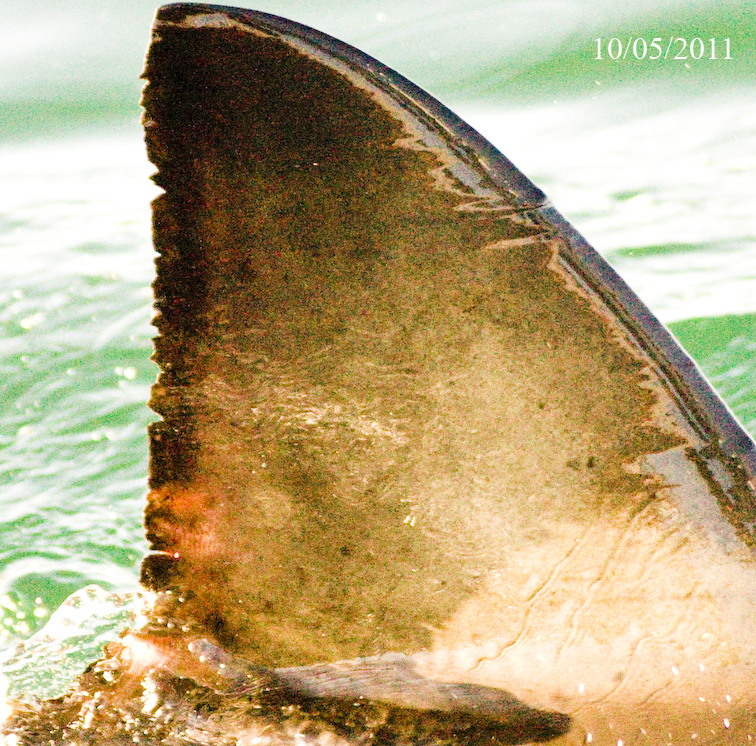
\includegraphics[width=2in]{haai1.jpg}} \quad
\subfigure[]{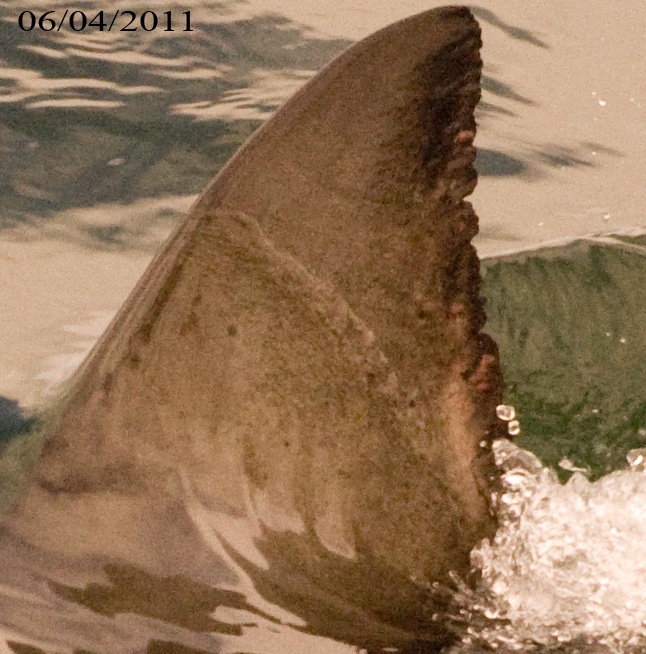
\includegraphics[width=2in]{haai4.jpg}} \quad
\subfigure[]{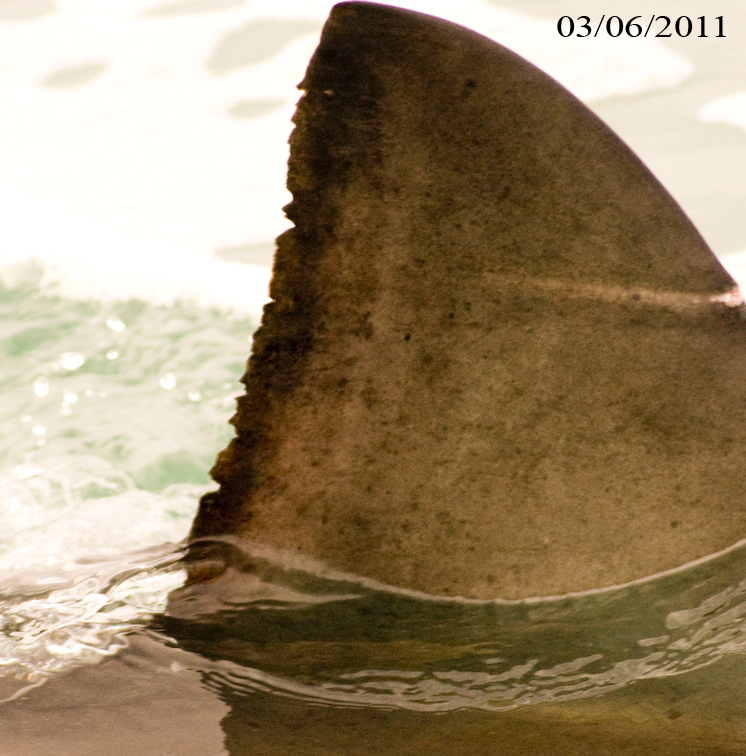
\includegraphics[width=2in]{haai2.jpg}}}
\end{figure}

\begin{figure}[H]
\centering
\mbox{\subfigure[]{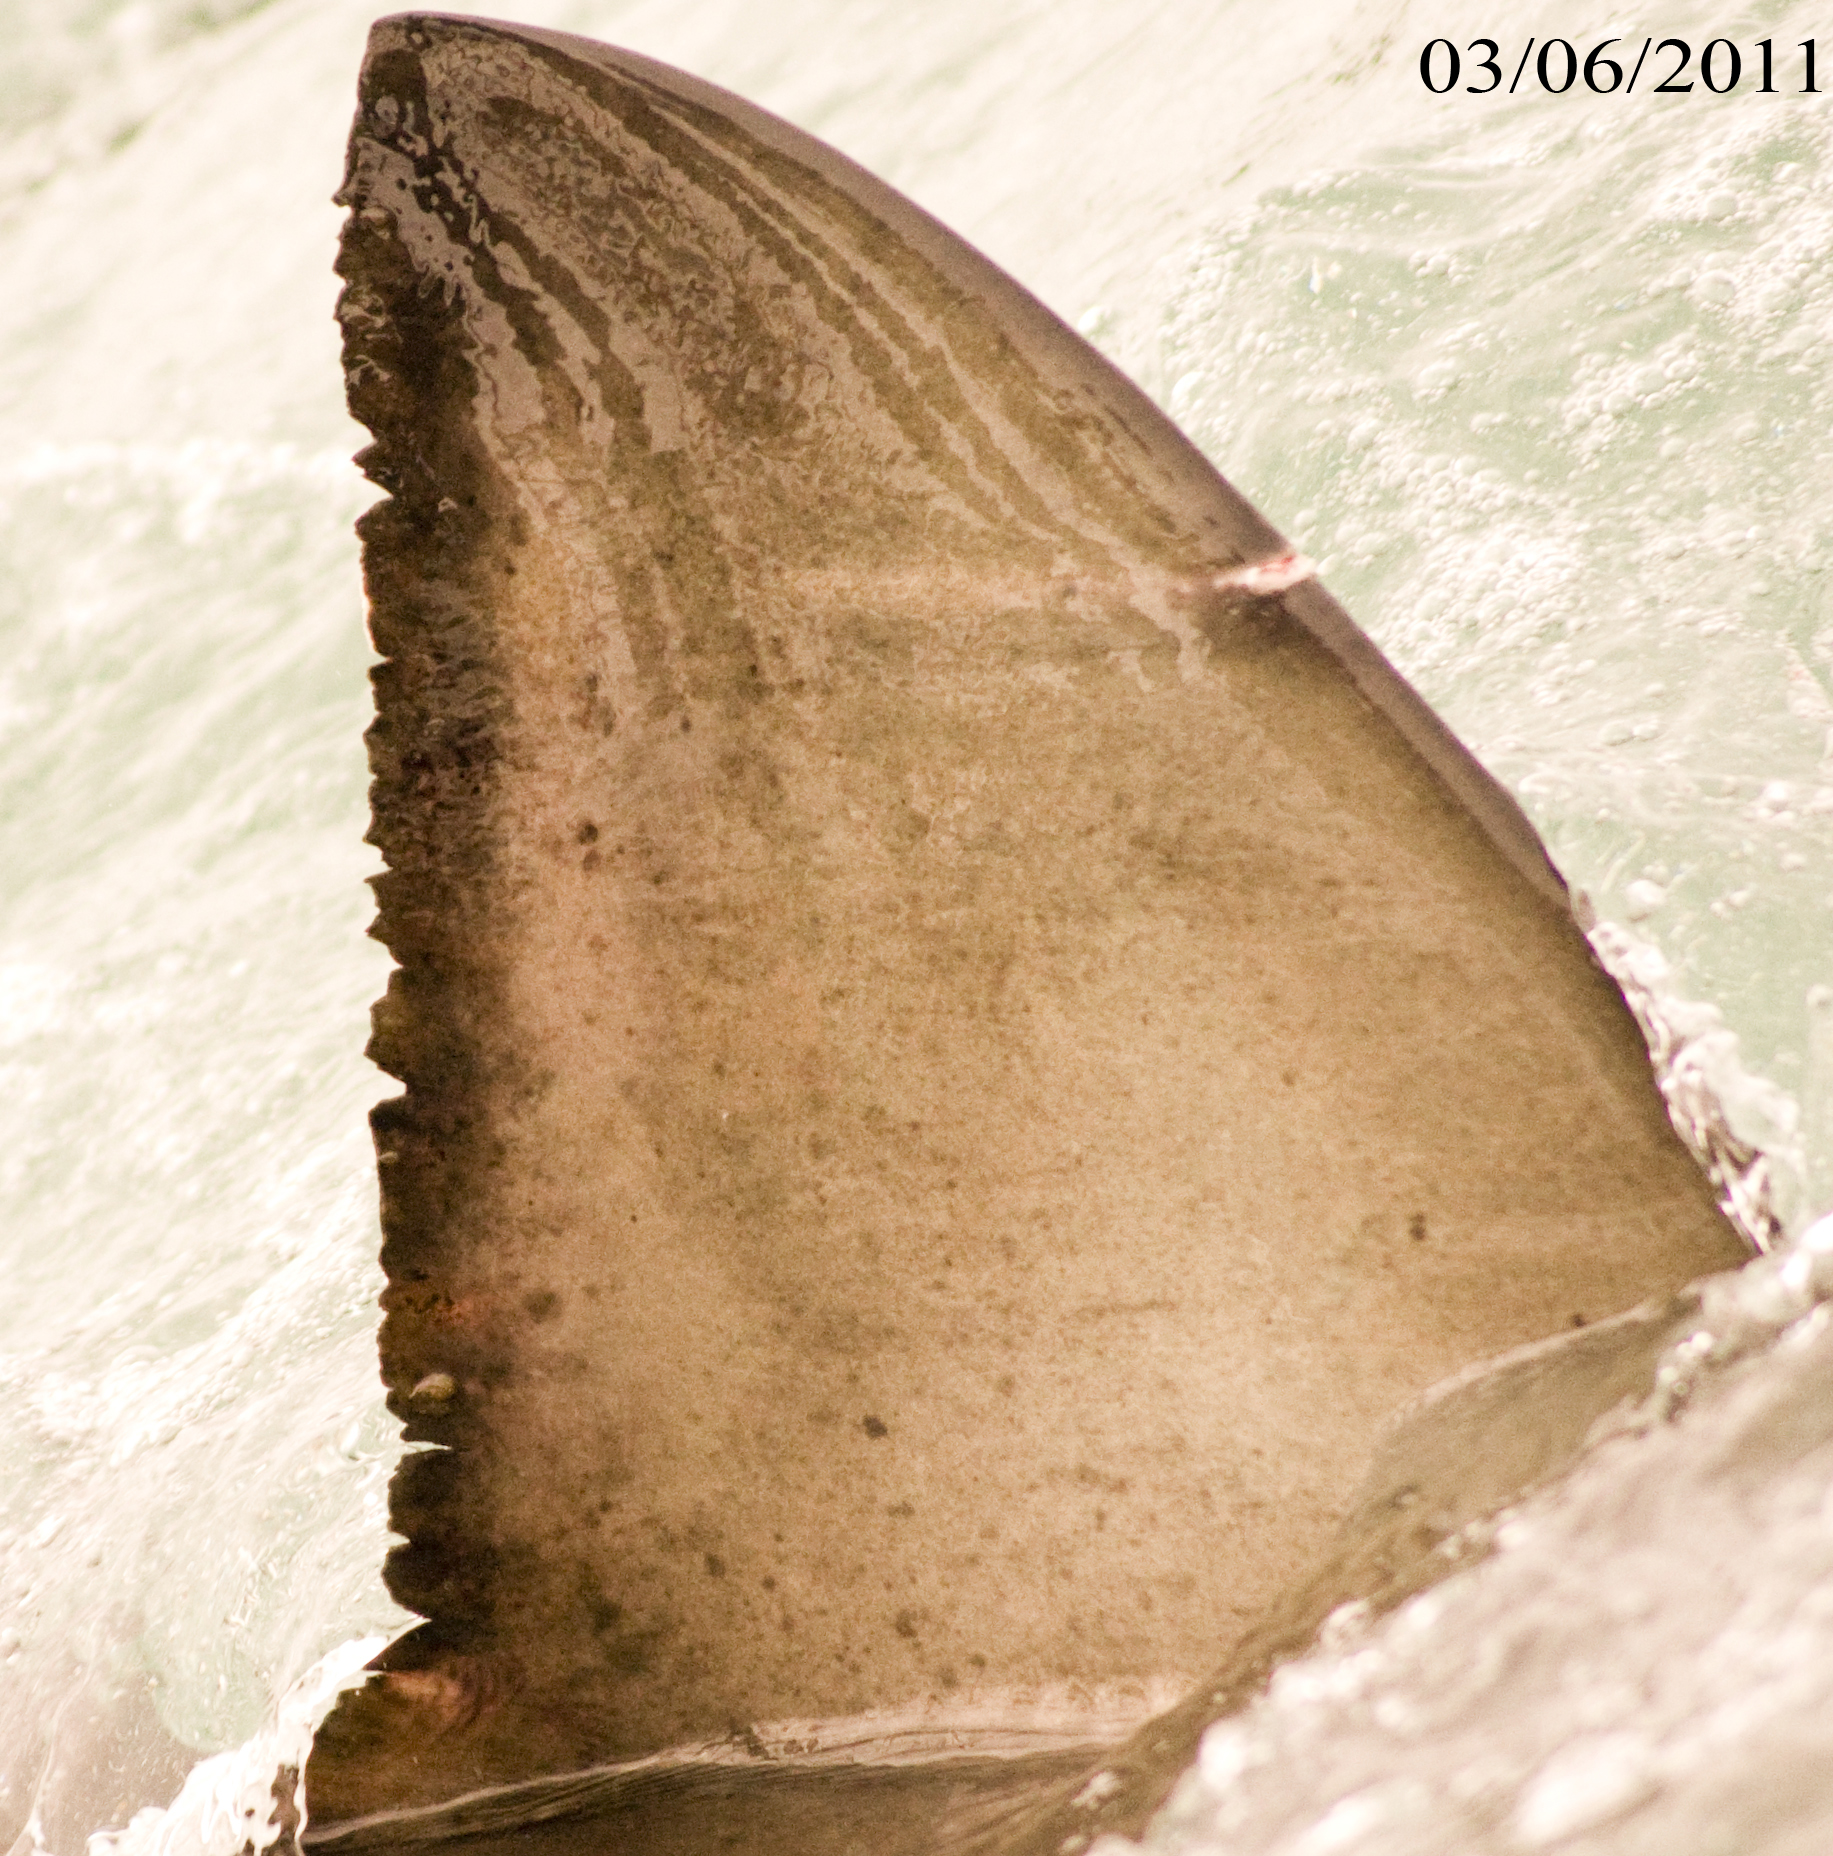
\includegraphics[width=2in]{haai3.jpg}} \quad
\subfigure[]{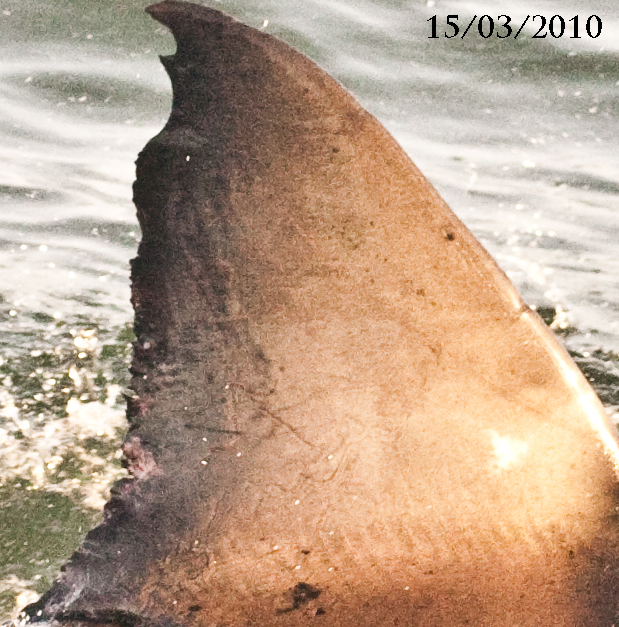
\includegraphics[width=2in]{haai5.jpg}} \quad
\subfigure[]{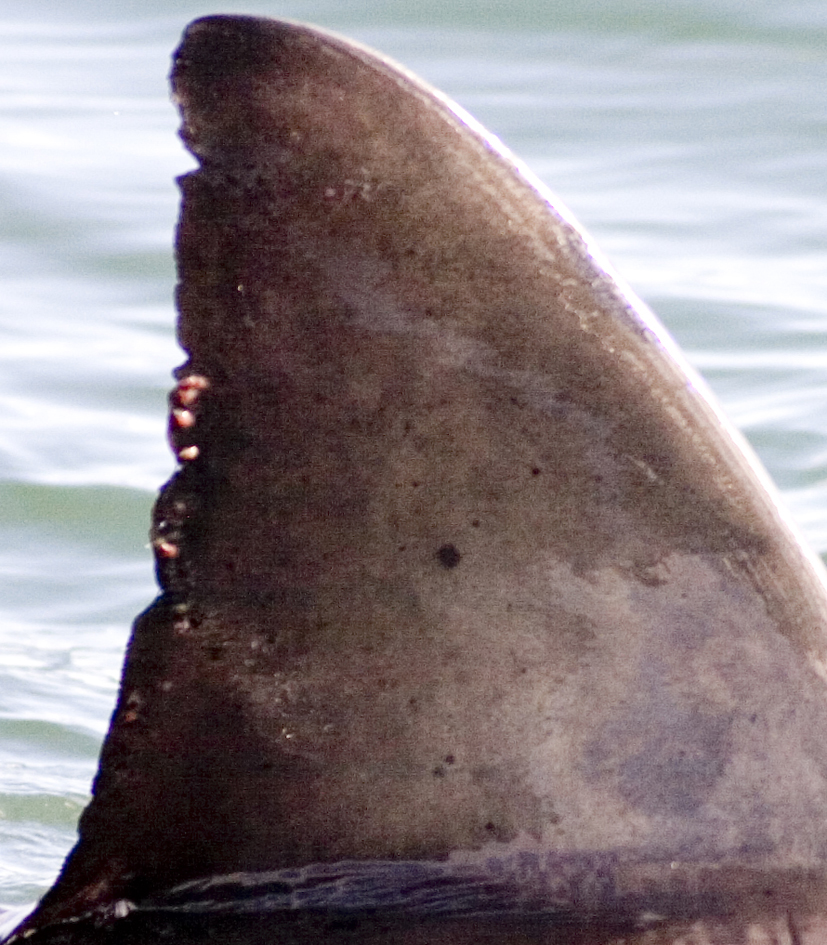
\includegraphics[width=2in]{haai6.jpg}}}
\end{figure}

\begin{figure}[H]
\centering
\mbox{\subfigure[]{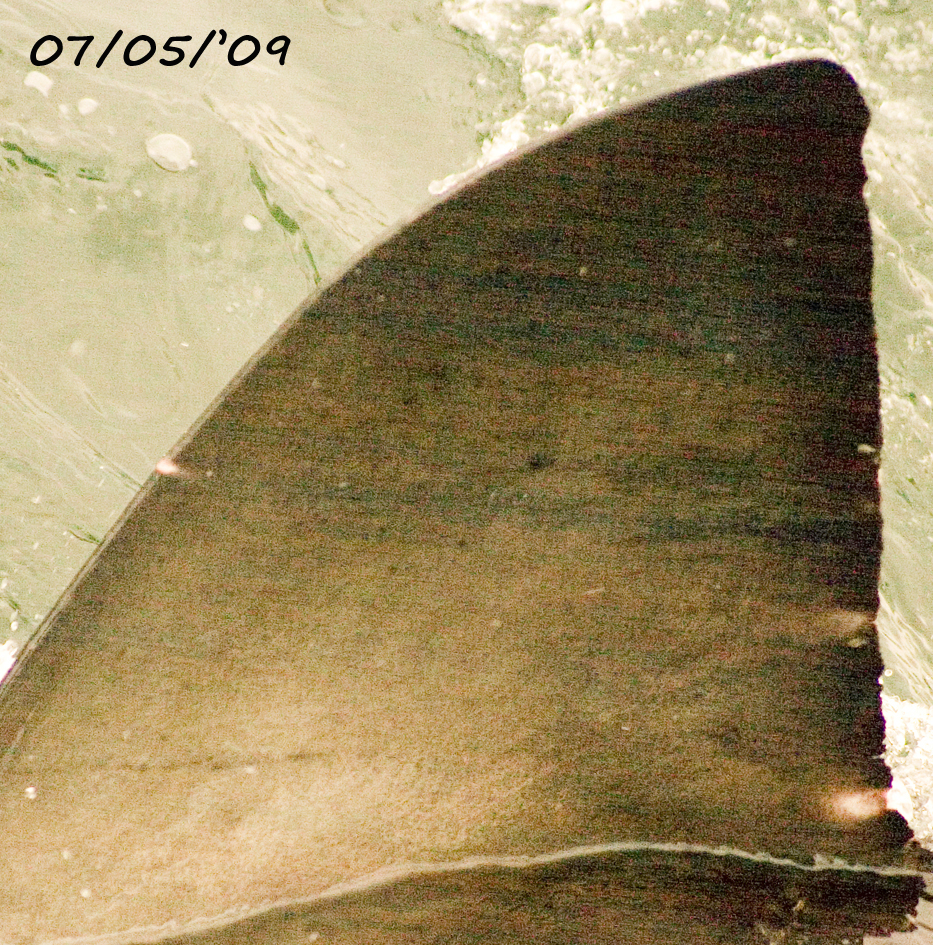
\includegraphics[width=2in]{haai7.jpg}} \quad
\subfigure[]{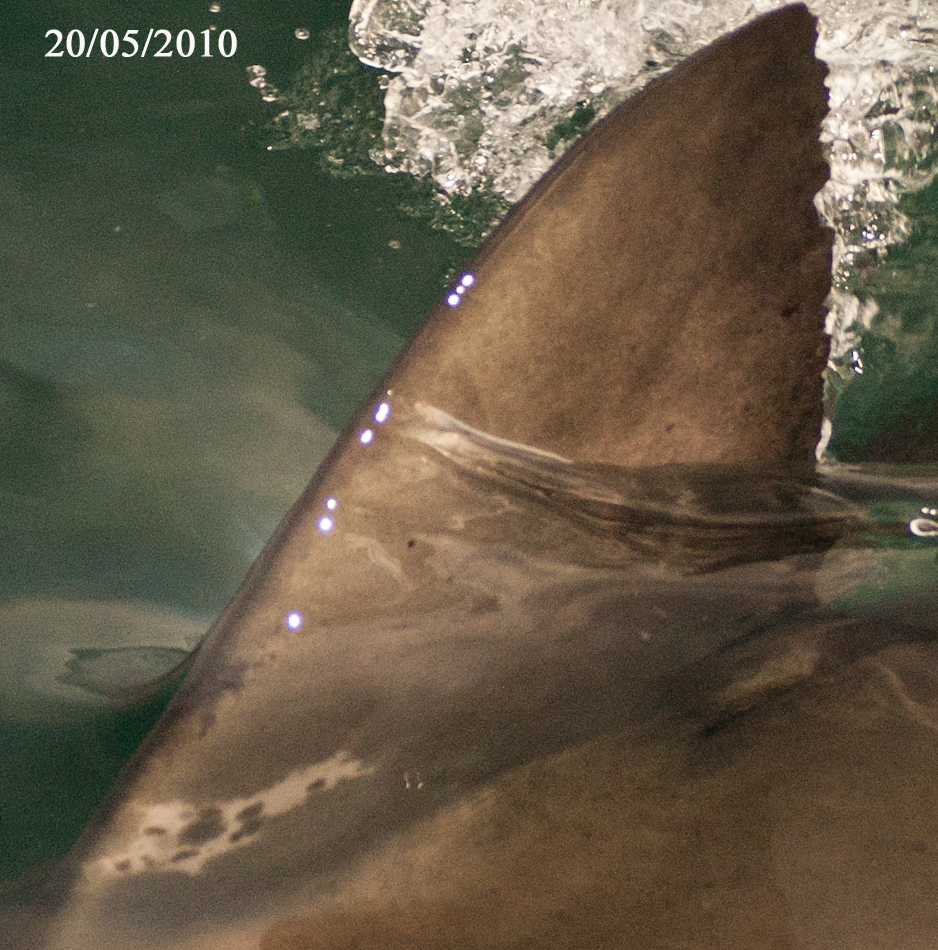
\includegraphics[width=2in]{haai8.jpg}} \quad
\subfigure[]{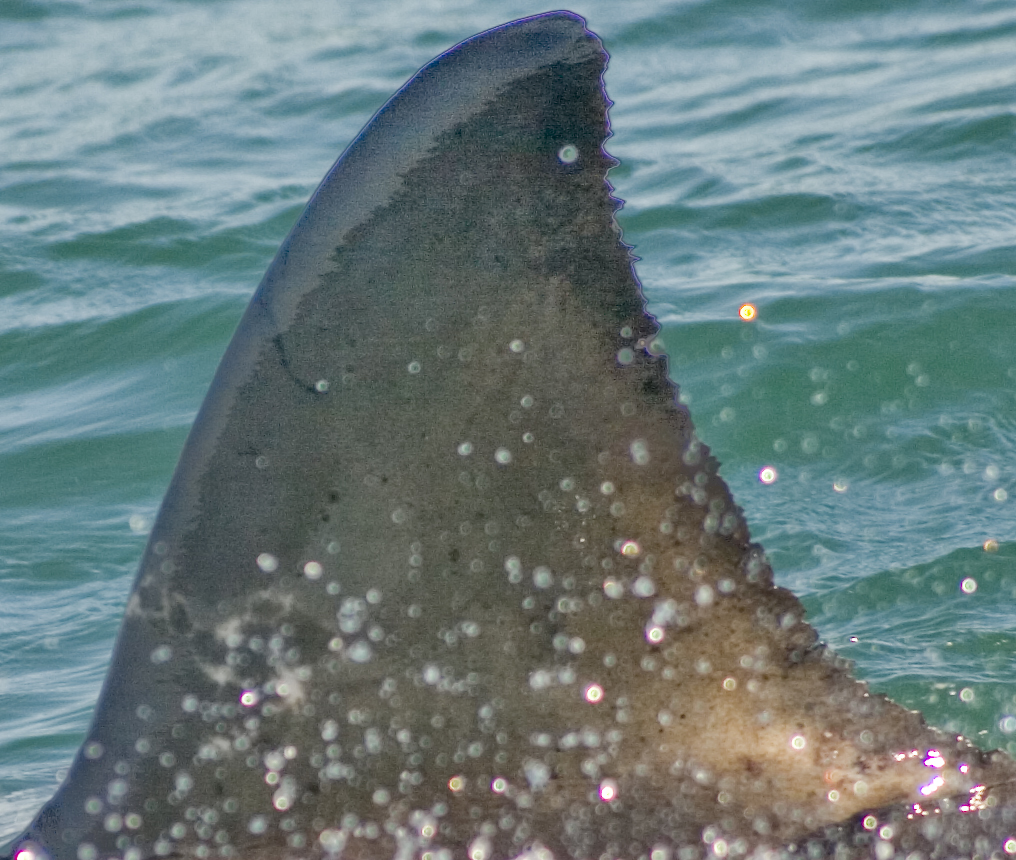
\includegraphics[width=2in]{haai9.jpg}}}
\end{figure}


\subsection{Background}
Image segmentation is commonly applied in image processing; it
aims to partition a digital image into multiple segments.
The image can then be interpreted using a smaller number of
well-defined components as opposed to a large array of unrelated pixels.  
In other words each pixel is assigned a label and all the pixels with the same
label share a certain
property, making the image easier to analyse. Image segmentation is
typically used to locate an object or boundaries in an image. \\

Segmentation algorithms can be classified as either supervised, meaning that
it requires user interaction, or unsupervised, meaning that it is totally
automatic.  Segmentation is a complex problem since computers must segment
an
image having only limited information about colour and space, for
example.
Furthermore, user interpretation is subjective since images can be ambigious and the goal of the segmentation indicates the robustness of the algorithm. 
Supervised algorithms need user input to make decisions.  On the other hand,
unsupervised algorithms need predetermined information and assumptions to work
automatically. \\

Well known examples where image segmentation is used is
in medical imaging to locate tumours, face and
fingerprint recognition and also in video surveillance.  See \ref{examples}.

\begin{figure}[H]
\centering
\mbox{\subfigure[]{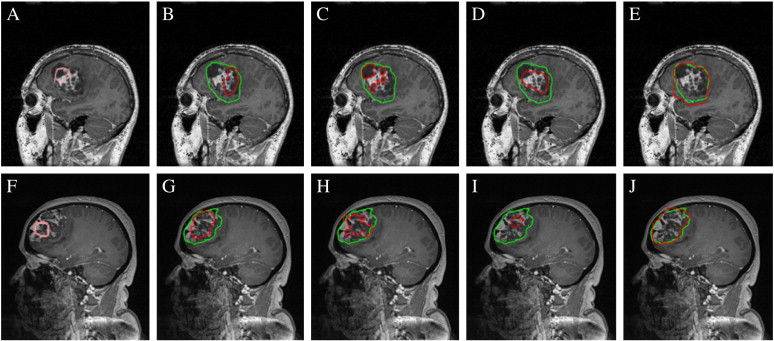
\includegraphics[width=2in]{braintumor.jpg}} \quad
\subfigure[]{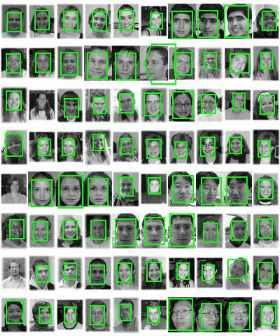
\includegraphics[width=2in]{face.jpg}}}
\caption{Image segmentation.}
\label{examples}
\end{figure}

Evaluating the segmentation outcome proves challenging.  It would be helpful to have a way for comparing
different
segmentation methods so that we know if progress is being made. 
The Berkeley Segmentation Dataset and Benchmark contains 12 000 hand-labelled
segmentations of 1 000 Corel dataset images by 30 human subjects. 
This can then be used to compare what humans think a good segmentation
should look like to computer analysis. \\

Here is an example of a colour image in the Berkeley Segmentation Dataset.  The image in the middle shows the machine segmentation and the
image on the right the human segmentation.

\begin{figure}[H]
\centering
\mbox{\subfigure[]{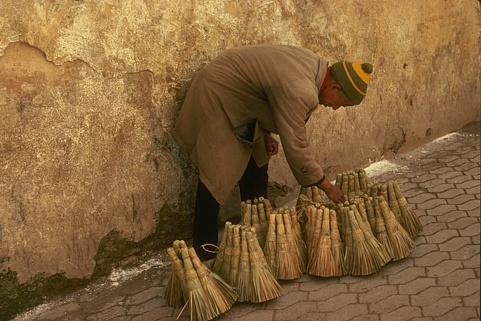
\includegraphics[width=2in]{data.jpg}} \quad
\subfigure[]{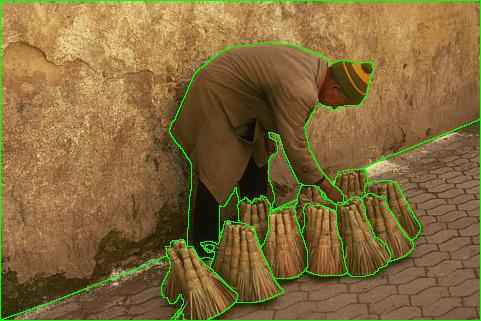
\includegraphics[width=2in]{data1.jpg}} \quad
\subfigure[]{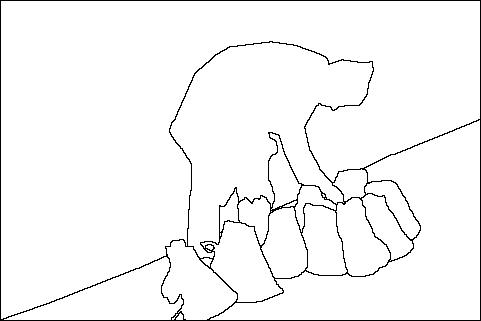
\includegraphics[width=2in]{data2.jpg}}}
\end{figure}

For the purpose of this research project, such datasets will not be used for
comparison of results.  A success rate, indicating the percentage of correct matches,
will rather be calculated.

\subsection{Software -- Python}
For the purpose of this research project, the Python Programming Language was
used.  Reasons for this are because of its simplicity, the powerful set of tools
available, and that it is easy to learn and understand.  Python is
also free to use and runs on multiple platforms.  For numerical and
scientific computations, Numpy and SciPy were used.
To improve the running time of implemented algorithms, Cython was used.  It is a
language that compiles to a Python extension module and a super set of the
Python language that allows calling C-functions and declaring C-types on
variables and class attributes.  This
results in the generation of efficient C-code from Cython code.
Scikit-image was used to investigate various image processing
techniques. \\

To ease collaboration, GitHub was used.  Github is a web-based hosting service
for software development projects.  This allowed us to easily
share code and documents and also quickly gather feedback.


\begin{figure}[H]
 \centering
 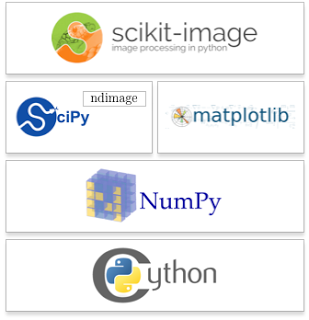
\includegraphics[width=3in]{logos.jpg}
\end{figure}

\newpage
\section{Overview of pipeline}
The procedure of identifying sharks can be
  divided into several components, together forming an image processing pipeline, each implemented as part of
  a bigger classifier.  The first algorithm is an orientation detection
algorithm that wil determine whether the shark fin is orientated to the left or the right in the image.
Then a segmentation algorithm will segment the shark fin from the image such that the path that defines the shark fin 
can easily be detected by the fin detection algorithm.  Thereafter a dynamic time warping algorithm is used
to compare the the paths that describe the fins and to see how shark fins in the databasis compare.
The various algorithms will now be discussed in detail.  Below is a diagram showing the structure of the pipeline.

\begin{figure}[H]
 \centering
 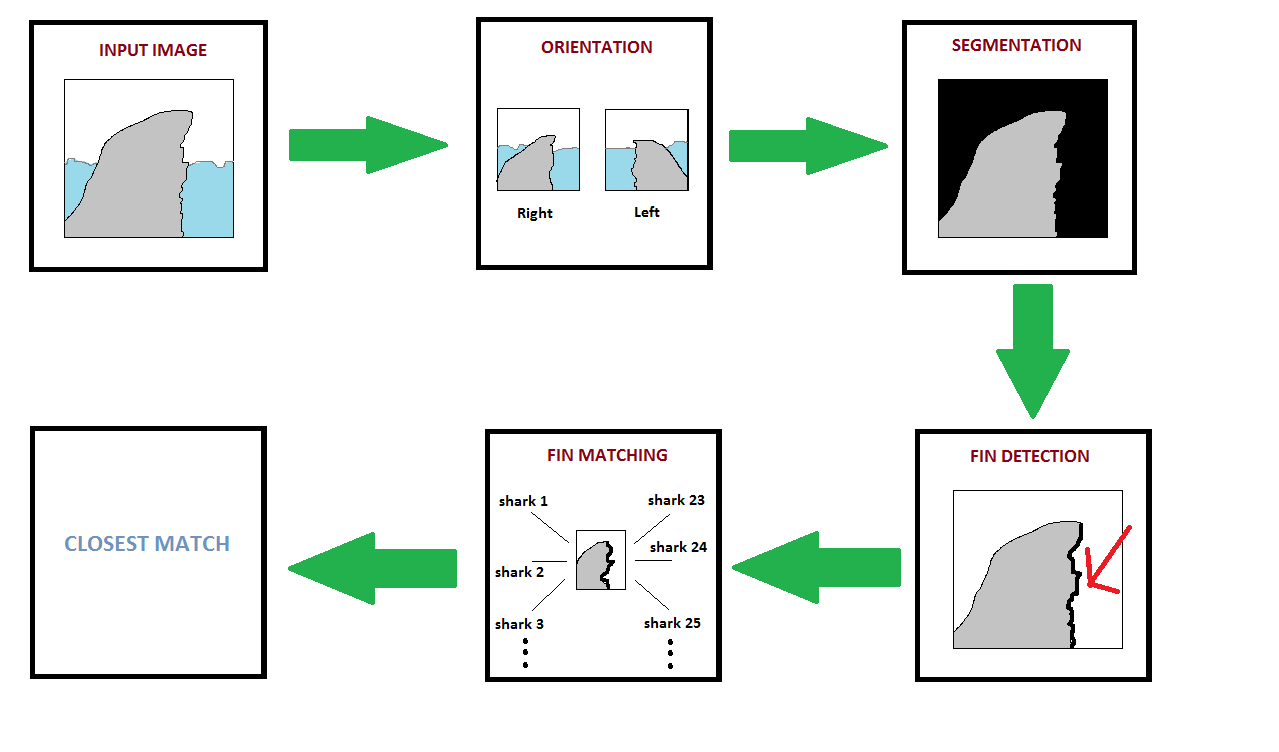
\includegraphics[width=5in]{pipeline.png}
\end{figure}

\note {Merge algorithm descriptions further down with this
section.  How??  What do you mean by this??}

\subsection{Orientation}
\label{orient}
To ease further analysis, the
orientation of the shark fin in the image is determined as the direction in
which the shark is
swimming, as viewed from the side, i.e., if the shark is swimming to the left,
the algorithm returns right and vice versa.  We then flip the images so that
all the shark fins have the same direction.  This will help when a few foreground
pixels and background pixels need to be specified when performing segmentation.
The method of Principal Components Analysis (PCA) is used here.  When applying
PCA, we are interested in finding the direction of maximum variation in the
data.  Suppose we have $K$, $n$-dimensional, data points, $\mathbf{x}_k,$ for
$k=1,2, \ldots ,K$.  We compute a covariance matrix, $C$, from our shark fin image as 
\[
 C_{\mathbf{x}} = \frac{1}{K} \sum_{k=1}^{K} \mathbf{x}_{k}\mathbf{x}_{k}^{T} -
\mathbf{m}_{\mathbf{x}}\mathbf{m}_{\mathbf{x}}^{T} 
,\]
where
\[
 \mathbf{m}_{\mathbf{x}} = \frac{1}{K} \sum_{k=1}^{K}\mathbf{x}_{k}
\]
is the mean of the data, computed along the columns of the shark fin image as an array. 
In our case, the data refers to the pixel values in the shark fin image.  \\

From $C$, we determine the eigenvalues and eigenvectors, which will indicate the
variance and principal directions respectively.
The direction of the eigenvector corresponding to the largest eigenvalue will
then indicate the orientation of the shark fin. \\

Below is a dummy shark fin image where the orientation is detected using PCA.
Note the principal axis, largest eigenvector, in blue, which gives the
orientation of the shark fin.
\begin{figure}[H]
 \centering
 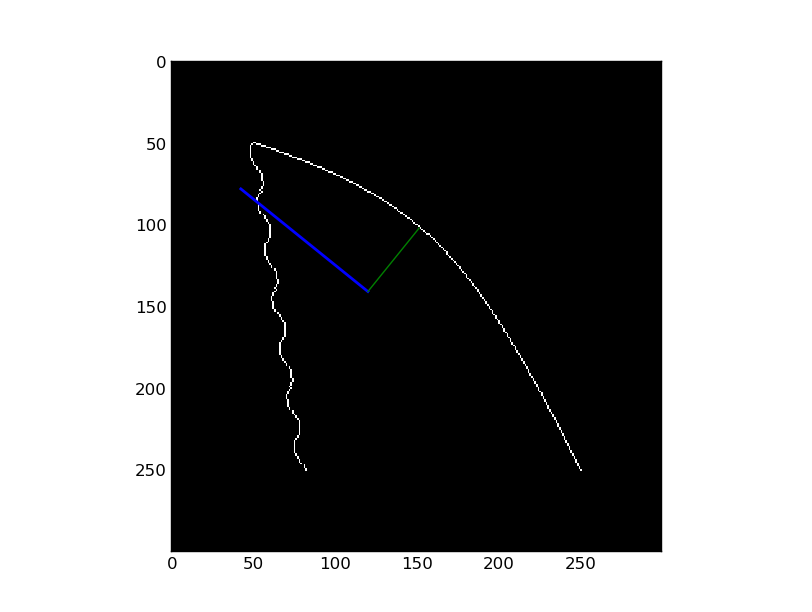
\includegraphics[width=4in]{orientation.jpg}
 \caption{Orientation of the shark fin detected by means of PCA.}
 \label{orientation}
\end{figure}

The above method is implemented by first converting the shark fin
image, which is an RGB image, to a grayscale image.  We then apply a Sobel filter
to identify prominent edges in the image.  After identifying the prominent edges
, we apply a threshold, using Otsu's method, to convert the image into a binary image.
We can now do PCA on
the image to determine the principal axes of the coordinates.  If the gradient
of the line defining the principal direction lies between 0 and
$\frac{\pi}{2}$ radians, the orientation of the shark fin is
identified as
"right", otherwise the orientation is identified as "left". 

\subsection{Segmentation}
\label{segmentation}
The task is to separate the foreground, the shark fin, from the background,
the sea.  For this purpose, we use the region growing segmentation algorithm,
Growcut (see \ref{growcut}).  Growcut requires the user to specify a few
foreground and background pixels from which the growing can be
initiated.\note{No description of growcut as an automaton?  Hoe kan ons die deel waar ek wel Growcut verduidelik hier in werk??}
Initially this was done by first determining the orientation of the fin (see
\ref{orient}) and then specifying a few pixels according to that, see 
\ref{segmentation}.  \\

\begin{figure}[H]
 \centering
 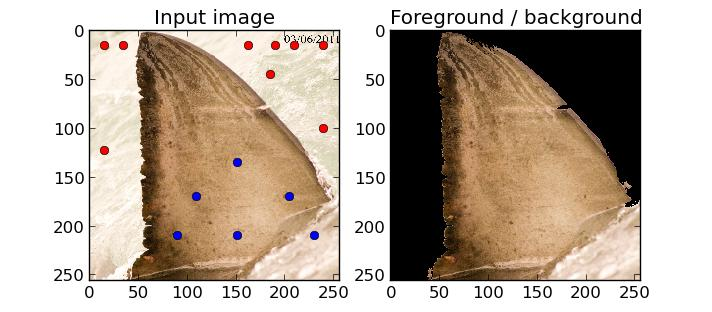
\includegraphics[width=5in]{segmentation.jpg}
 \caption{Growcut segmentation on a shark fin image by selecting a few
foreground and background pixels, shown in blue and red respectively.}
 \label{segmentation}
\end{figure}

The specification of
the foreground and background pixels is done using the function
\texttt{grid\_points\_inside\_poly()} from the \texttt{morphology} module in
\texttt{scikit-image}.  This function selects all points inside a given
polygon.  These selected  points are then set as the initial foreground and background pixels
respectively.  See
\ref{segmentation1}.
Since the images in the database, and images in general, are not
all the same size, we specify the corners of the polygon according to the size
of the image.  This then makes the algorithm more robust.  \\

\begin{figure}[H]
 \centering
 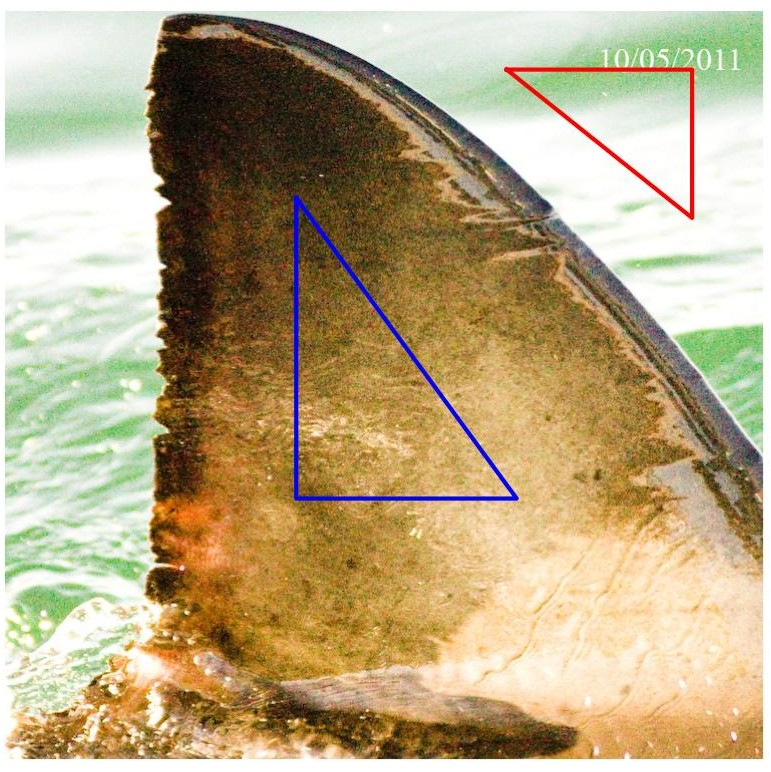
\includegraphics[width=2.6in]{polyshark.jpg}
 \caption{Growcut segmentation on a shark fin image by selecting all points in a
given polygon as foreground and background pixels, shown as blue and red
 polygons respectively.}
 \label{segmentation1}
\end{figure}

Now that we have specified a few foreground and background pixels, we also
need to specify the size of the neighbourhood around cells when the algorithm
is 'growing' as well as the number of iterations the algorithm should follow.
These parameters inevitably influence the success of the
segmentation.\note{The reader cannot follow this explanation without knowing
how growcut works.  Hoe kan ons dit hier bywerk???}
\\

Below is an example of the final output of the segmentation process. \\
\note{show at different stages, perhaps? Agree!}

\begin{figure}[H]
 \centering
 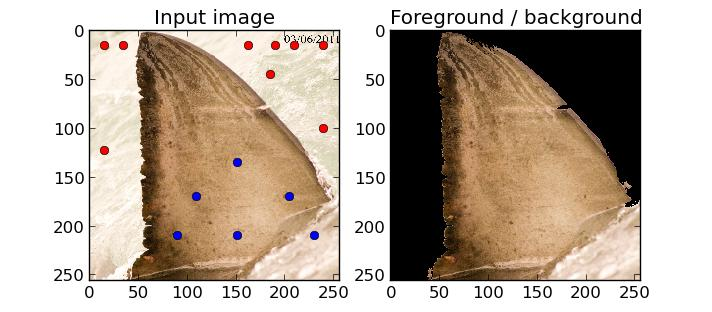
\includegraphics[width=5in]{segmentation.jpg}
 \caption{Segmented shark fin image.}
 \label{segmentation1}
\end{figure}

At the moment the segmentation algorithm is running at a very low speed.
This then slows down the whole process of identification.  We can either cache 
the results so that future requests for data can be served faster, 
or we can leave out the segmentation process.  The latter will then result in
finding the path defining the fin directly from the edge image.

\subsection{Fin detection}
The objective is to identify the serrated part of dorsal shark fin. In order to
do this, we need to extract this part of the fin, so that it is in a form to be 
compared with other fins easily.  We use the
Sobel operator,
well-known in edge detection, to identify edges in the image and ease further analysis.
The sobel operator is a discrete differential operator that approximates the
gradient of the image intensity function.  It uses two different $3 \times 3$
masks, $M_x$ and $M_y$, which are convolved with the original image to
approximate the
derivatives, both in the horizontal $x$-
and the vertical $y$-directions.  \\

Define $A$ as the input image and $G_x$ and $G_y$ as the gradient images in the
$x$-and $y$-direction respectively,
after convolving with $A$.  $M_x$ and $M_y$ is given by

\[
 M_x = \begin{pmatrix*}
        1 & 0 & -1 \\
        2 & 0 & -2 \\
        1 & 0 & -1
       \end{pmatrix*}
\mbox{ , }
 M_y = \begin{pmatrix*}
        1 & 2 & 1 \\
        0 & 0 & 0 \\
        -1 & -2 & -1
       \end{pmatrix*}
.\]

At each point in the image, the gradient approximations can be combined to give
the gradient magnitude image, calculated  as
\[
 G = \sqrt{G_x^2+G_y^2}
.\]

The sobel operator applied to one of the shark fin images is shown in
\ref{sobel}.  Note that this operator only works on a grayscale image.
We can see the edge of the fin in the $G$ image on the right clearly identified.

\begin{figure}[H]
 \centering
 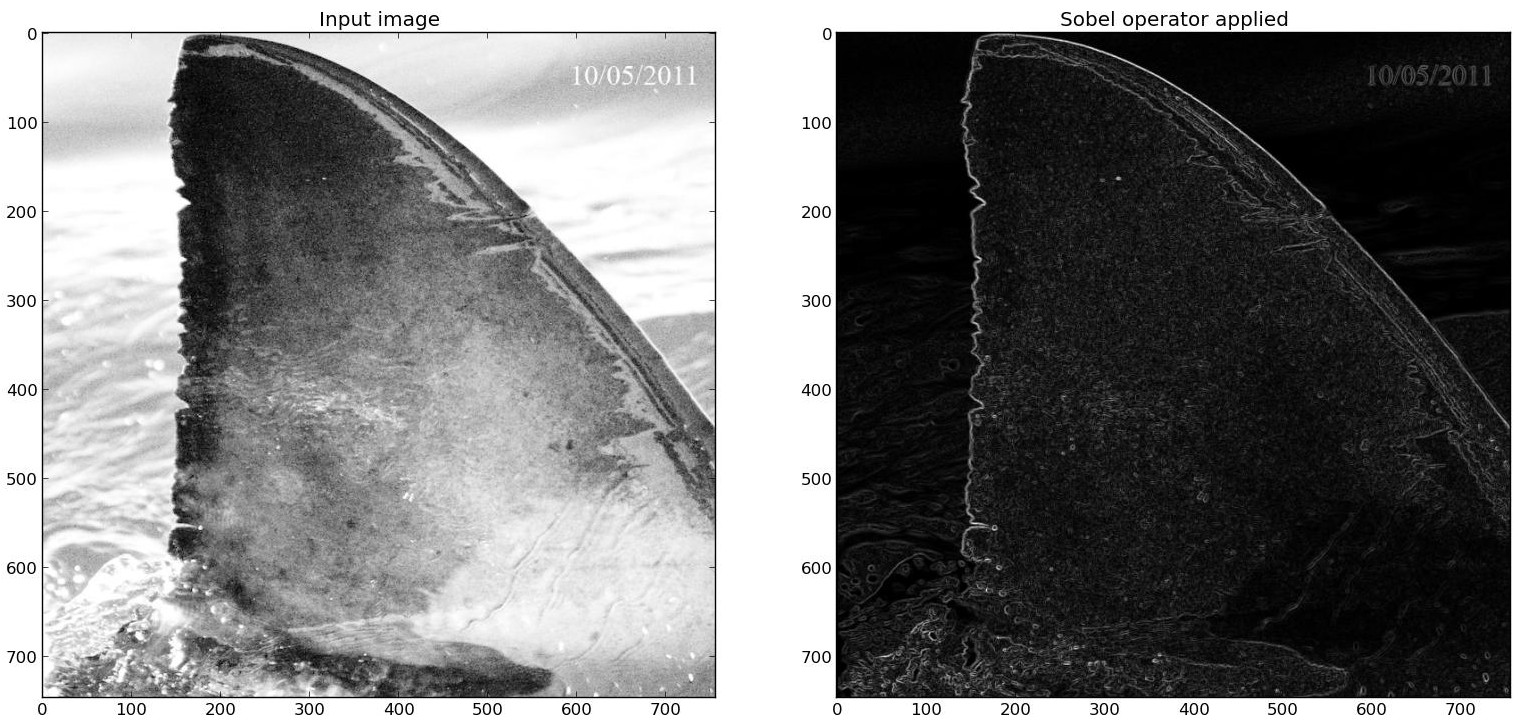
\includegraphics[width=5in]{sobel.jpg}
 \caption{The Sobel operator.}
 \label{sobel}
\end{figure}

The next step is to extract only the unique part of the fin needed for
identification.  This is done by first inverting the edges and then squaring
them to increase their weight and thereby making them more prominent.  We make use of a function 
\texttt{route\_through\_array()} from the module \texttt{graph} in scikit-image.
 This function enables us to find a lowest cost path through the image.
Since we are working on the segmented image, we allow any start and end point
for the path.\note{How do we do that?}  The path is computed by ??????.  All
pixel coordinates running on the edges of the image is then removed from the
path.\\

Here we show an example of the path, in blue, that was detected on the shark
fin.
\begin{figure}[H]
 \centering
 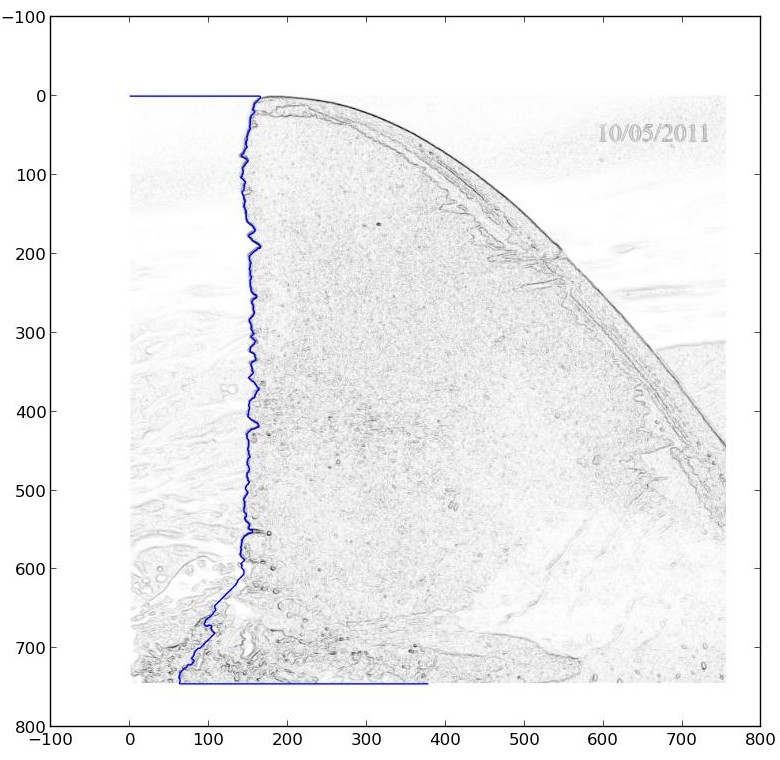
\includegraphics[width=3in]{path.jpg}
 \caption{Fin path detected.}
 \label{fin}
\end{figure}

Images such as the one below poses a great challenge when finding the path defining the dorsal fin.
Since the reflection of the fin on the water is so prominent, the path which is detected by this algorithm also
picks up the reflection.  We are therefore unsure as to where the path starts and ends.  This can be corrected by either making sure the reflected part will be segmented out as background or by shifting the path over the fin and detecting drastic changes in pixel values.

\begin{figure}[H]
 \centering
 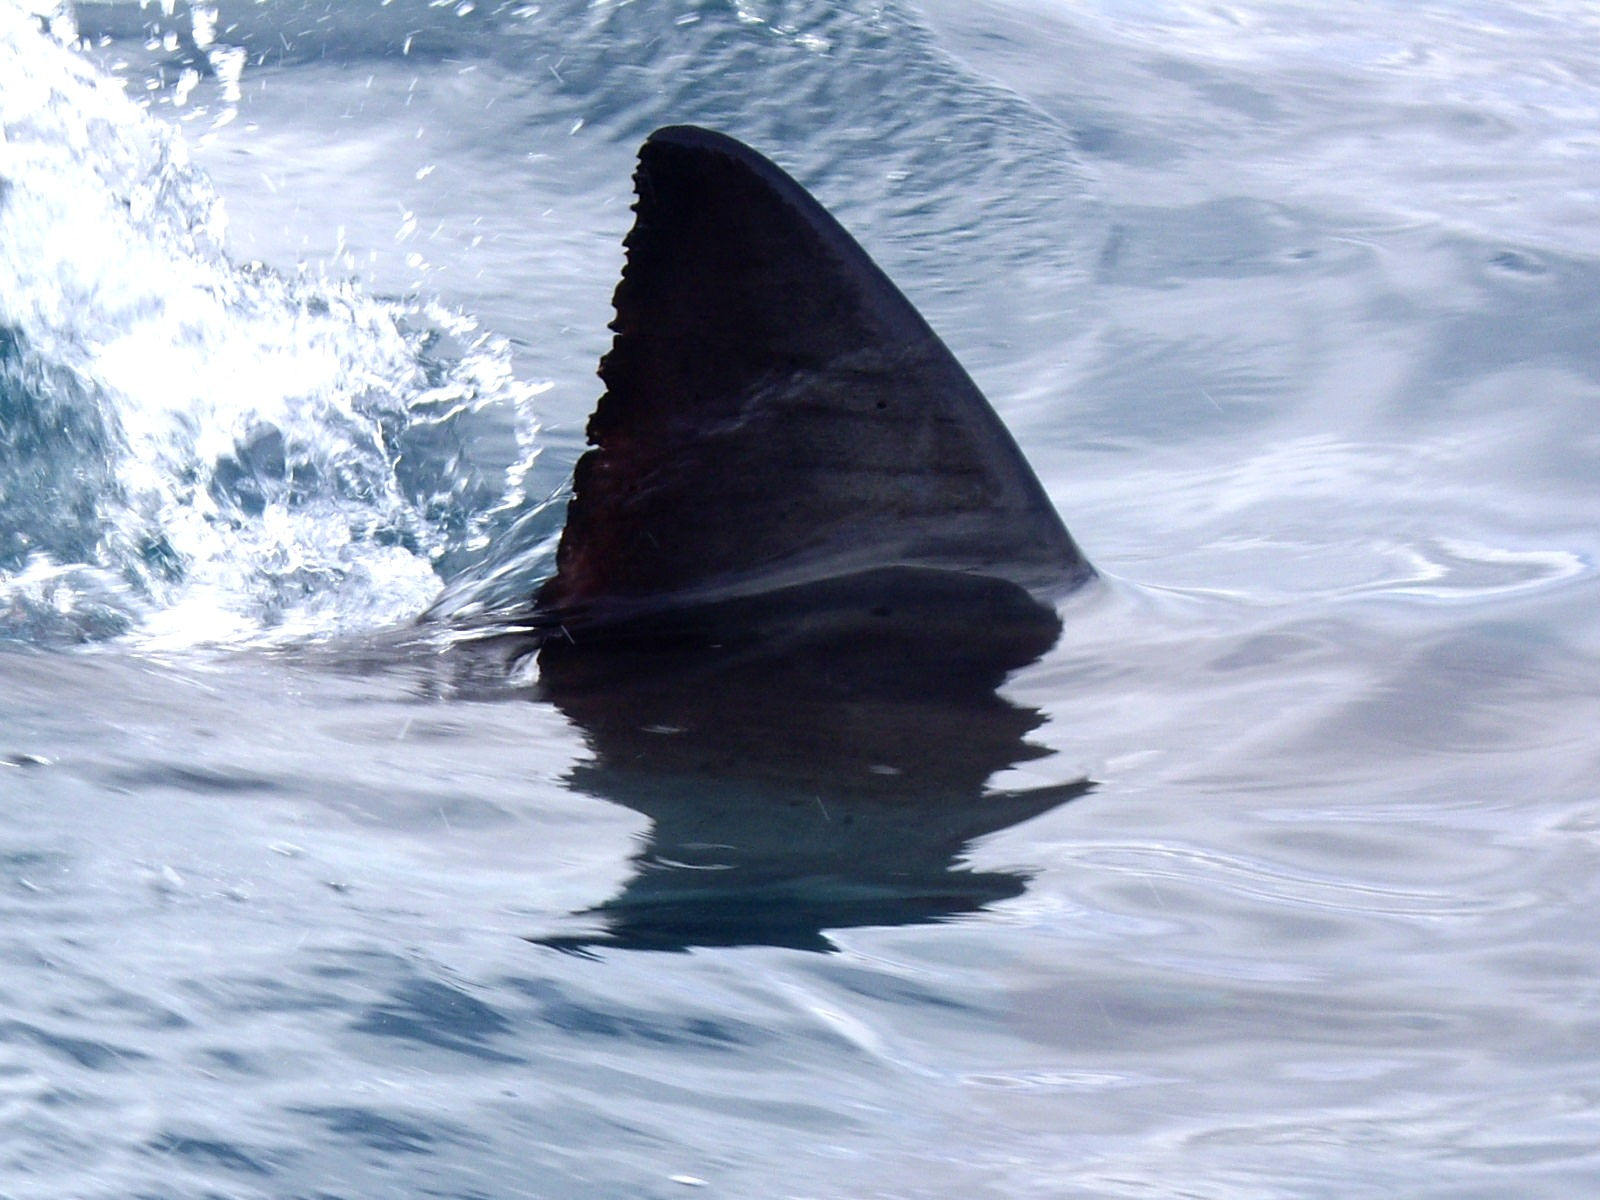
\includegraphics[width=3in]{reflectfin.jpg}
 \caption{Note the prominent reflection of the dorsal fin in the water.}
\end{figure}

\subsection{Fin matching}
Dynamic time warping (DTW) is an algorithm used for
measuring the similarity between two sequences which may vary in time or
speed.  It differs from normal comparison in the
sense that it accommodates sequences of different lengths, warping the
sequences for the best fit to be compared.
Any data that can be represented linearly can be analysed using DTW.  \\

When comparing two sequences, a typical approach is to calculate the distance
between corresponding points.  The Euclidean metric can be used
to calculate this distance, but
it assumes that the $i$-th \note{wys dat dit 'n inskrywing $A_ij$ vorm. Verstaan nie???} point in
the first sequence will align with the $j$th point in the second sequence.
But
since the sequences need not be
the same length, we will make use of a non-linear alignment\note{Hoe moet ek dit verduidelik???}.

A distance matrix is calculated, containing the difference between
each pair of elements in the array as entries.  We now view this matrix as a
grid, where the
aim is to find a lowest cost path from the top left corner of the grid to the bottom right
corner of the grid.  Thereby making sure that each element in the array is compared to every other element in the array.
The minimum cost is then a measure of the similarity between the
sequences.
In other words, the lower the cost, the less the sequences differ and the greater the match.
\\

\begin{figure}[H]
 \centering
 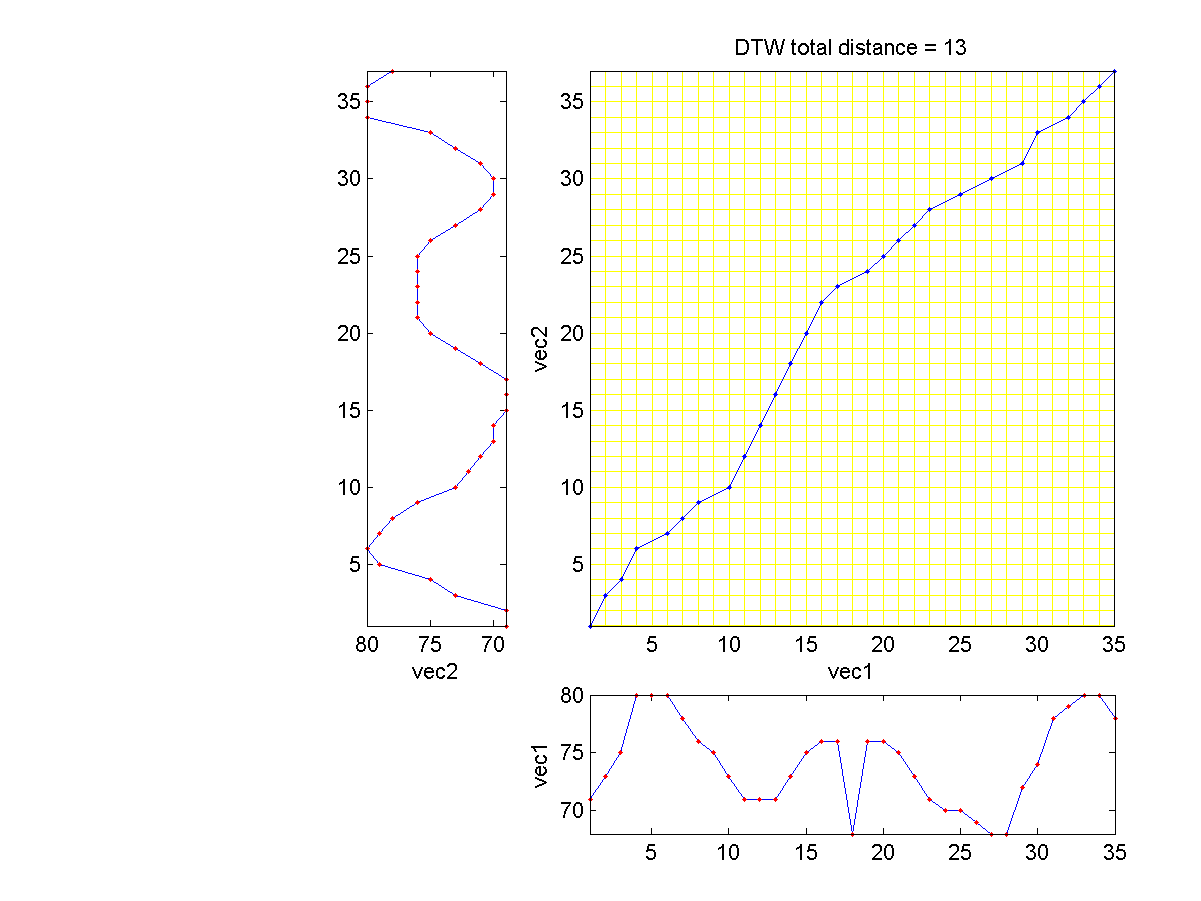
\includegraphics[width=4in]{dtw1.png}
 \caption{.}
 \label{dtw1}
\end{figure}

For this part of the pipeline, the output from the fin detection method,
\note{diagram! Van wat???}i.e.
the coordinates of the path defining the shark fin, is used as input.  The DTW
method will follow the above procedure to compare every shark fin to every
other shark fin in the database, each time returning a minimum cost.  
Thus for a database containing $N$ shark fin images, a $N \times N$ cost
matrix will be returned, where the entry in $(i, j)$ corresponds to the cost
of the path when shark fin $i$ is compared to shark fin $j$.  We then identify the shark
corresponding to the minimum of these entries in a specific column. \\


Below is an example where two arrays are compared using DTW. Note the lines
connecting the points being compared.  
\begin{figure}[H]
 \centering
 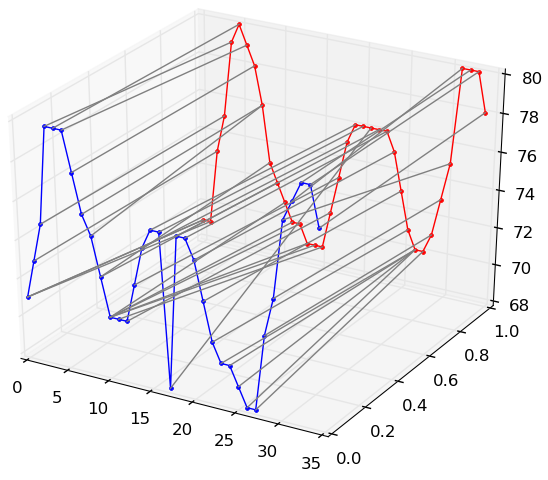
\includegraphics[width=3in]{dtw.jpg}
 \caption{Fins compared as arrays.}
 \label{dtw}
\end{figure}

\newpage
\subsection{DARWIN -- Alternative software}
The DARWIN\cite{Darwin} software package is well known when it comes to
aquiring important data about dolphins.  It was initially implemented
by undergraduate student of
Eckerd College.
Lately it was used to estimate the Great White shark population in the
Gansbaai area by means of shark fin identification and matching.  They claim to
have found approximately
1008 different shark species in this region.  This
claim was tested by Ms. S. Andreotti, using a database of 50 shark fin images and she found that in only
54\% of the cases, the correct matching took place, making this software
unreliable.

\begin{figure}[H]
 \centering
 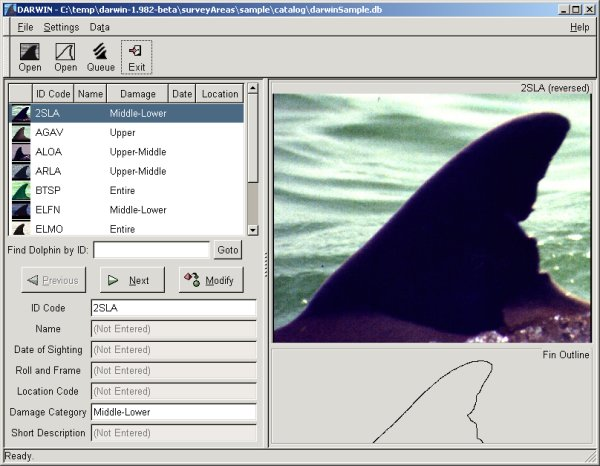
\includegraphics[width=3in]{Darwin.jpg}
 \caption{DARWIN user interface}
\end{figure}

In this research project, we test our software on the same set of 50 shark fin images to make more reliable conclusions.
Since our software is specifically aimed at the identification of sharks, a first attempt at identification will at least 
give a lower bound for the success rate.

\newpage
\section{Segmentation Algorithms}
\subsection{Different categories and techniques}
Segmentation algorithms can be arranged into different categories \cite{is}. 
Some of the most well-known categories are
\begin{itemize}
 \item \textbf{Thresholding}  Thresholding is an unsophisticated method. It
relies on
     selecting a good threshold
     value, using Otsu's method for example, to convert a gray-scale image into
a binary image.  Segmentation is
     then done on the binary image. 
 \item \textbf{Clustering} For these methods, the $K$-means algorithm
can be used to partition an image into $K$ clusters, whereafter
segmentation will follow.
 \item \textbf{Compression-based} This method conjectures that the
optimal segmentation is the one that minimizes, when considering all possible
segmentations, the coding length of the data. In other words, the number of bits
required to encode that image, based on the given segmentation.
 \item \textbf{Histogram-based}  This is a very efficient method in the
sense that it only passes through all the pixels once.  A histogram of 
the image is computed whereafter the peaks and valleys in the histogram
are used to locate clusters in the image.  Here clusters refer to pixels
sharing a certain property.  The colour or intensity of the pixels can be used
to
locate clusters.
 \item \textbf{Edge detection} Edge detection is well researched in image
processing.  Region boundaries and edges are closely related,
since there are usually a sharp adjustment at region boundaries.  Edge detection
techniques can therefore be used as a bases for different segmentation
algorithms.
 \item \textbf{Region growing} This method takes as input not only
the image, but also a set of seeds, which marks the objects to be segmented. 
Thereafter neighbouring, unallocated pixels are compared to the specific seed
point.  That is how the region grows iteratively.  The pixels are compared using
the difference between intensity value and the region's mean.  Pixels are then
allocated to a specific region if that difference is a minimum.  The process
terminates if all pixels belong to a a specific region.  \note{This is not
accurate, I
don't think.  Region merging is all about merging *regions*.  Don't
understand??}
 \item \textbf{Watershed transformation} See description in \ref{watershed}.    
 \item \textbf{Graph partitioning} This method is based on modelling
the image as a weighted, undirected graph, where the nodes represent the pixels
and the weights represent the similarity between neighbouring pixels. Then the
graph is partitioned into clusters according to a specific criterion.  Each
partition is then considered an object segment in the image.
 \item \textbf{Trainable} Also known as Neural network segmentation,
this process involves processing the small areas of an image by means of an
artificial neural network or a set of neural networks.  Thereafter, using the
categories recognised by the network, the decision-making mechanism marks the
image accordingly and segmentation is done.
\end{itemize}

\subsection{Cellular automaton}\note{Hoe kan ek hierdie deel met die Growcut deel integreer?? Want dit verg kennis van wat ek onder 
Growcut verduidelik.}
The idea of an cellular automaton is explained with the use of an example.
Probably the most well-known example of a two dimensional automaton is Conway's
Game of Life, developed by British mathematician John Horton Conway in 1970. 
This "game" is a zero-player game, i.e. it developes according to an initial
state
and require now further input.  The "player" interacts by creating an initial
state whereafter evolution of cells take place.  \\

The space in which the game takes place can be described as an infinite
two-dimensional grid of square cells.  Each cell can be in either one of two
states, dead or alive.  In Conway's Game of Life, each cell interacts with the
cells in its eight-neighbourhood or Moore neighbourhood.  The following rules are 
used to update the sate of each cell.  Note that these rules will differ for each automaton. 

\begin{itemize}
 \item  Any living cell with less than two living neighbours, will die because of under population.
 \item Any living cell with two or three living neighbours lives on to the next generation.
 \item Any living cell with more than three living neighbours dies because of over population.
 \item Any dead cell with exactly three living neighbours becomes a living cell, because of reproduction.
\end{itemize}

New generations are created by applying these rules simultaneously to every cell and therefore births and deaths occur simultaneously. \\

Below is an example of different structures created by different rules, all following the procedure described above.

\begin{figure}[H]
\centering
\mbox{\subfigure{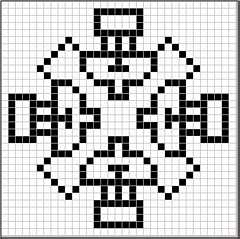
\includegraphics[width=2in]{conway2.jpg}} \quad
\subfigure{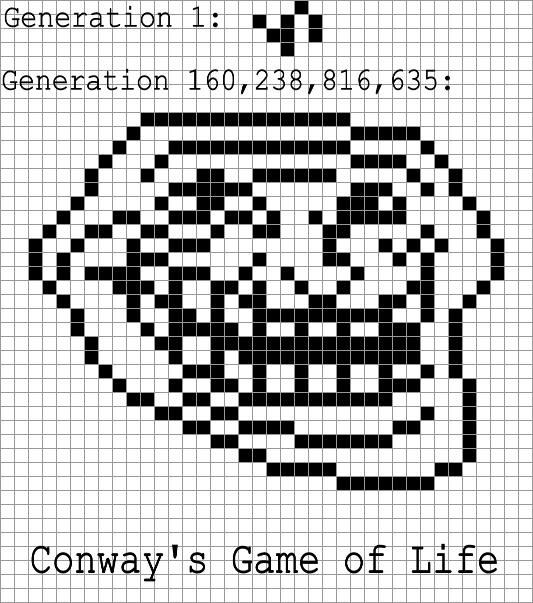
\includegraphics[width=2in]{conway1.png}}}
\caption{Some interesting patterns formed by different cellular automaton.}
\end{figure}

\subsection{Growcut}
\label{growcut}
The Grow Cut algorithm is an interactive, multi-label segmentation algorithm
for N-dimensional images.  The algorithm is based on cellular automata, i.e.,
the user labels a few pixels and the rest of the image is then segmented
automatically by a cellular automaton.  A cellular automaton consists of a
grid of cells, where each one of the cells can be in a finite number of
states, say on and off.   Around each cell, a set of cells, called the cell's
neighbourhood is defined.  An initial state, at time $t = 0$, is also assigned
to each cell.
A new generation of cells is then created according to a fixed rule or
mathematical function that determines the new state of the cell, by looking at
the current state of the cell as well
as that of its neighbourhood.  Two of the most common neighbourhood systems used are the Von
Neumann neighbourhood and the Moore neighbourhood which are shown below.
This rule
is then applied to all of the cells simultaneously.  In this way, the cell's
state gets updated.  Note that the rules for updating the state of each cell are
the same and do not
change over time. \\

\begin{figure}[H]
\centering
\mbox{\subfigure{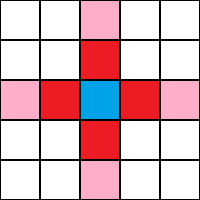
\includegraphics[width=1.7in]{VonNeumann.png}} \quad
\subfigure{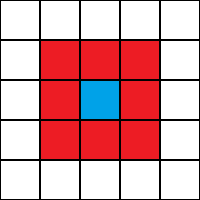
\includegraphics[width=1.7in]{Moore.png}}} \caption{Von Neumann and
Moore neighbourhood systems \cite{n}}
\end{figure}

The algorithm is interactive, since the user can observe the segmentation and
guide the algorithm in places where the segmentation is difficult to compute.
\\

\noindent The basic method on which the algorithm relies is the following.  A
cellular automaton is an algorithm which is discrete in both space and time
and operates on a lattice of pixels $p \in P \subset Z^{n}$.  A cellular
automaton can be considered as a triplet, $A = (S, N, \delta)$, where $S$ is a
set containing different states, $N$ is the
neighbourhood system of the cell and $\delta: S^{N} \rightarrow S $ is a
transition rule.  This is the function which defines  the rule calculating the
cell's state at time $t + 1$, given the states 
of the cell's neighbourhood at time $t$.  Two well known neighbourhood systems
are the von Neumann and Moore neighbourhood systems.  The cell state referred to
is also
considered a triplet $(l_{p}, \theta_{p}, \overrightarrow{C}_{p})$, where
$l_{p}$ is the label of the cell($K$ labels in total), $\theta_{p}$ is the
'strength' of the cell and $\overrightarrow{C}_{p}$ is
the cell feature vector.  Without loss of generality it can be assumed that
$\theta_{p} \in [0,1]$. 

The initial state of the pixels is set to $l_{p} = 0, \theta_{p} = 0,
\overrightarrow{C}_{p} = RGB_{p}$, where $RGB_{p}$ is a three dimensional vector
of the pixel's colour in 
the RGB space.  The goal of the segmentation is to assign one of the possible
$K$ labels to each one of the pixels.  The user starts the segmentation by
marking specific pixels as foreground and others as background.  This sets the
initial state of each pixel.  While the labels are being updated, the user can
correct and guide the process if desired.  \\

\newpage
\noindent The pseudo code for the automata evolution rule is shown below. 
\begin{algorithm}[H]
\begin{algorithmic}[1]
 \State // For each cell...
 \For{$\forall p \in P$}
 \State // Copy previous state
 \State $l^{t+1}_{p} = l^{t}_{p}$;
 \State $\theta_{p}^{t+1} = \theta_{p}^{t}$;
 \State // Neighbours try to attack the current cell
 \For{$\forall q \in N(p)$}
 \If{$g(\| \overrightarrow{C}_{p} - \overrightarrow{C}_{q} \|_{2}) \cdot
\theta^{t}_{q} > \theta_{p}^{t}$}
 \State $l^{t+1}_{p} = l^{t}_{q}$
 \State $\theta^{t+1}_{p} = g(\| \overrightarrow{C}_{p} - \overrightarrow{C}_{q}
\|_{2}) \cdot \theta^{t}_{q}$
 \EndIf
 \EndFor
 \EndFor
\end{algorithmic}
\end{algorithm}

\noindent where $g$ is a monotonous decreasing function bounded to $[0, 1]$. 
The function is given by
\[
g(x) = 1 - \frac{x}{max\| \overrightarrow{C} \|_{2}}. 
\]


\noindent The algorithm has been modified in the following way.  One of the
main features that needed attention was the damping function $g$.  By changing
the exponent of the term $\frac{x}{max\| \overrightarrow{C} \|_{2}}$ to
$\frac{3}{2}$, thus $\left ({\frac{x}{max\| \overrightarrow{C} \|_{2}}}\right
) ^\frac{3}{2}$,
an immediate result was seen.  The algorithm acted much more accurately around
the edges.  Next, the 'defend strength' of each pixel was modified also by
playing with exponents
of certain parts of the code.  A
sobel filter was used in detecting the edges.  A sobel filter calculates the
gradient of the intensity of each pixel, giving
the direction of the largest possible increase from light to dark and also the
rate of change in that specific direction.   This results in showing how
abruptly or smoothly the images changes at that point and then how likely it
is that that part represents an edge.  The figure below shows a sobel filter
acting on a shark fin image.  The edges of the shark fin can clearly be seen.
The main purpose of these changes was to improve accuracy when detecting the
edges.  \\


\noindent Here is a comparison between the effect of the original algorithm on
one of the shark fin images and the effect of the modified version of the
algorithm on the same image.
\begin{figure}[H]
 \centering
 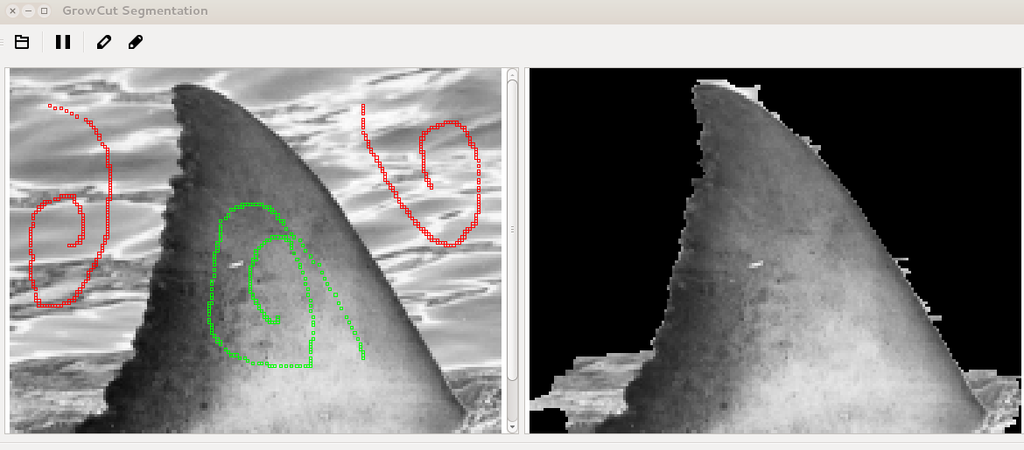
\includegraphics[width=4in, height=1.8in]{haaio}
 \caption{The effect of the original algorithm}
 \label{fin1}
\end{figure}

\begin{figure}[H]
 \centering
 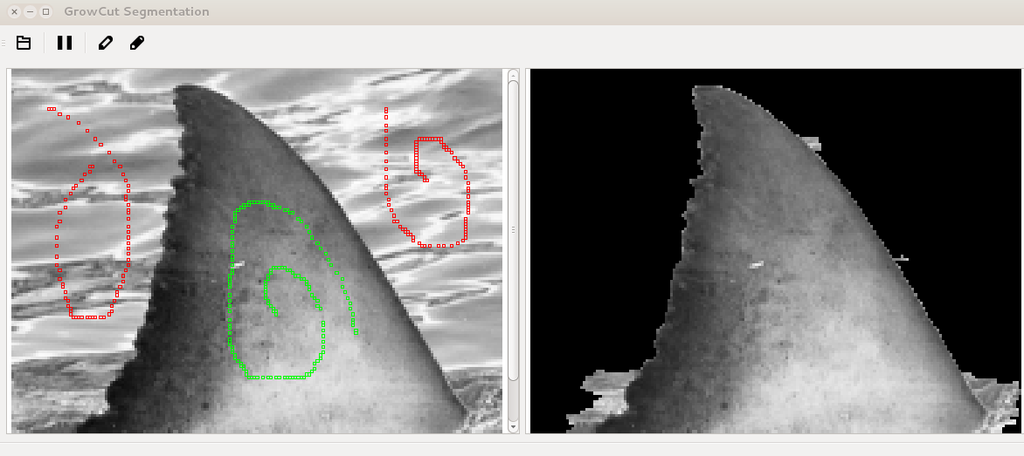
\includegraphics[width=4in, height=1.8in]{haaim}
 \caption{The effect of the modified algorithm}
 \label{fin}
\end{figure}

\noindent It can be seen that the modified version gives better results around
the edges, which is essential in the case of the shark fin images. \\ 

Hoe kan ek hierdie deel inwerk??????

First consider reducing the running time.  One way is to look at which cell
features, i.e. difference in intensity combined with cell strength and cell
strength alone, play a more important role in updating the cell label, i.e.
foreground or background.   This will then help in finding 
redundant conditions in the code.  By eliminating those conditions the running
time can be reduced.  It is concluded that neither of the before
mentioned features can be omitted, although cell strength alone has a more
significant role in finding the new cell label.  No new 'attacking' 
strategies have yet been implemented. \\

The use of a rank filter is also being investigated.  A rank filter looks for
the cell with maximum intensity in a certain region, specified by the user, 
and assigns that intensity to the cell it is being compared to.  This will
better the way in finding the cells in a certain region with intensities that
is much different from the intensity of the cell being considered. \\  

\noindent From \cite{RF} we conclude the following.  The semantic segmentation
algorithm is based on pixel wise object segmentation.  This is done by 
assigning category labels to a set of super pixels obtained by clustering the
joint colour space and coordinate space using the mean shift algorithm.
The method of interactive semantic segmentation as in \cite{RF} can be described
as follows.  Each image is presented as a set of super pixels, where 
a super pixel is a set of pixels.  The first image in the data set must be
segmented manually by labelling each super pixel.  An appearance model is 
now created.  The next image is now segmented automatically using the appearance
model.  During the segmentation the user may correct mistakes by 
relabelling and thus updating the appearance model.  Every time the user
approves the segmentation, the system learns from the new labelling information.
As image segmentation continues, user time spent on correcting labels reduces
and thus the rate of image labelling increases.  \\

This method can be helpful in the sense that it works with a database of images
of the same kind.  Since the shark fin images are all of the same type, 
it would be very beneficial to manually segment the first image only and then
automatic segmentation will follow.  By updating the appearance model, 
one can also be certain that better segmentation results will follow.  \\  


\subsection{Random Walker}
The method, as
described in \cite{rw}, is as follows.  The user labels a few
pixels as foreground or background for example.  This is then called the seeds. 
A random walker is then released from each of the unlabelled pixels. 
Thereafter, the probability that a certain pixel's random walker first arrives
at a specific seed, is computed.\note{Look at the scikit-image gallery on
random walker to see how they explained it.  Got this from the reference they
gave there.}  In other words, if the user
labels $n$ pixels, each with a different label, then the probability that a
random walker
leaving the pixel will first arrive at a certain seed, must be
computed.  The latter is done by modelling the image as a weighted graph, where
the weight of an edge reflects the similarity(intensity values) between pixels,
and then solving a system of linear equations.  The pixel is then assigned the
label
of the seed for which it is most likely to reach.  The process is repeated until
each pixel is assigned a specific label. 


\subsection{Watershed}
\label{watershed}
Another segmentation algorithm is the classic watershed algorithm, as
implemented in \cite{scikit}.  The algorithm starts with user-defined markers,
called seed points, which can be viewed as little holes in the image, whereafter
pixel values are treated as a topography/landscape.  The algorithm then floods
basins from the user-defined markers until basins which attribute to different
markers meet at watershed lines.  In this case marker positions are chosen as
the local maxima of the image.  Thereafter the segmentation is done on the
gradient image.  The result of the watershed algorithm applied to a shark fin
image is shown below.

\begin{figure}[H]
\centering
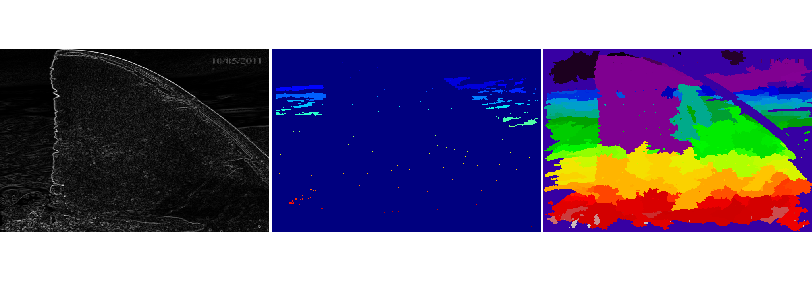
\includegraphics[width=5in,height=2in]{watershed.png} 
\label{fig1}
\caption{The watershed algorithm.}
\end{figure}

\noindent The first image shows the gradient image of the original shark fin
image.  The second image shows the pixels that are identified as a local maxima.
 The third image shows how the basins flooded until watershed lines are reached.
 Putting the correct segments together, which will require a lot of hard work,
an effective segmentation can be done.

\subsection{Graphcuts}
Graphcuts is a technique to select the best quality segmentation.  In doing so,
we calculate a global optimum solution by minimizing a certain 
cost function.  One of the reasons for the success of graphcuts is because of
the way the cost is defined.  It is a combination of what each pixel
"wants" and what is "best" for its neighbourhood.  We define an ergy function,
$E$, to determine the cost of a specific segmentation.
\[
 E = \sum_{p \in \Phi}E_d(p) + \lambda\sum_{p,g \in \Phi}E_n(p, q)
\]
where the term $E_d(p)$ is the cost of assigning pixel $p$ label $d$, the
neighbourhood term $E_n(p, q)$ is the difference in cost of labels for pixels
$p$ 
and $q$, and finally $\lambda$ is a weighting parameter to specify the
importance of either term.

\begin{figure}[H]
 \centering
 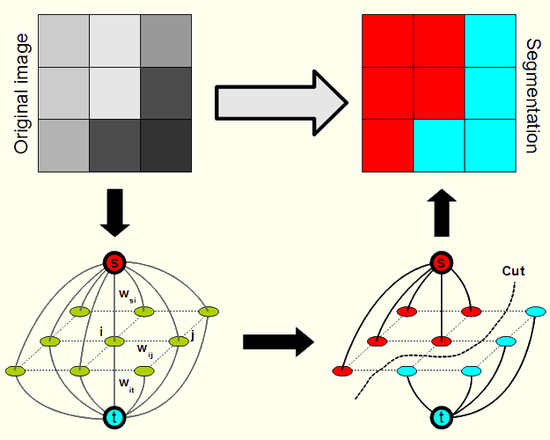
\includegraphics[width=3in]{graphcut.jpg}
 \caption{.}
\end{figure}


\newpage
\section{Results}
\subsection{}


\subsection{}


\subsection{}


\newpage
\section{Conclusions}
\subsection{Research, Wat moet hierdie opskrif wees????}
Initially this research project entailed studying different segmentation algorithms with the idea to be able to identify sharks for various environmental and biological reasons.
A request from a PhD student for assistance in her research project on identifying sharks led to the development of a pipeline. The Growcut algorithm was used as the main segmentation algorithm. A workable pipeline was developed. \\





\subsection{}


\subsection{Future work}
Future work can include developing an user interface, making the identification of shark fins more user friendly and user interactive.
An user, who must be connected to some database of shark fins, will be able to use this interface, containing the different parts of the pipeline, to identify shark fins.  Each part will consist of an interactive "window".  The different parts of the pipeline can be used separately, in conjunction with each other or as a whole.  New shark fin images can then be uploaded, from which various ecological and behavioural information can be extracted.

For example, the segmentation window will allow the user to manually select foreground and background pixels as described in \ref{segmentation}.
When performing the algorithm, the user can guide the process by selecting more pixels for segmentation. \\

Another aspect that needs investigation is the fact that the algorithms are not running at optimum speed.  This then poses the challenge of speeding it up.  Cython can be considered as a possibility to rectify this. \\

The pipeline must also be tested using a wider variety of segmentation algorithms, for example graphcuts. This will then help in choosing the most successful segmentation,
meassured by the amount of correct matches it produces. \\ 

After the classification of shark fins is done, it would be valuable if one could "cluster" different sharks according to fin similarities.
One could then try to recognize various families of sharks. \\

\newpage
\bibliography{final}

\end{document}
